% !Mode:: "TeX:UTF-8"

\documentclass[11pt, a4paper]{article}
%\usepackage{xltxtra,fontspec,xunicode}
\usepackage{amsmath}
\usepackage{amssymb}
\usepackage{breqn}
\usepackage{autobreak}
\usepackage{braket,mleftright}
\usepackage{amsfonts}
\usepackage[section]{placeins}
\usepackage{float}
\usepackage{siunitx}
\usepackage{graphicx}
\usepackage{subcaption}
\usepackage{fixltx2e}
\usepackage{mwe}
\usepackage{indentfirst}
\usepackage{caption}
\usepackage{physics}
\usepackage{geometry}
\usepackage{graphicx}
%\usepackage{caption}
%\usepackage{subfigure}
\usepackage{algorithm}% http://ctan.org/pkg/algorithm
\usepackage{algpseudocode}% http://ctan.org/pkg/algorithmicx
\usepackage[numbers,sort&compress]{natbib}

\geometry{top=1in, bottom=1in, left=1in, right=1in}
%\linespread{1.5}

\DeclareMathOperator*{\argmax}{argmax}
\DeclareMathOperator*{\argmin}{argmin}

\newcommand{\degc}{$\,^\circ$C}

\begin{document}

\title{Non-equilibrium RNA Folding as an Evolutionary Basis of E. Coli 5'-UTR Codon Bias}
\author{Zhuoran Qiao}
\date{\today}

\maketitle

\section{Introduction}

\paragraph{1} Developed GenoFold, a novel approach to simulate kilobases level co-transcriptional folding kinetics.
\paragraph{2} Quantitatively investigated the dependence of transcient Shine-Dalgarno accessibility on mRNA level variation within a synonymous mutant library.


\section{Method development}
\subsection{Framework}
Various algorithms or programs have been developed to predict RNA folding pathway ultilizing force-field based simulations\cite{RaviprasadAduri2007}
and multiple sampling methods based on Monte Carlo trajectories\cite{Gultyaev1995}\cite{Clote} or coarse graining of energy landscape built on Markov state model\cite{Wolfinger}\cite{Sun2018}. Those present methods have succeeded in revealing multiscale dynamic events during RNA folding, however are either designed for only predicting annealing dynamics or limited to RNA segments with length up to hundred bases.

To quantitatively predict folding dynamics coupled with transcription, we developed GenoFold, a genetic algorithm and Markov state model (MSM) based approach, which is capable of capturing kilobase level kinetics. This method is composed of a recombination step to generate configuration states in the MSM from historical information, a propagation step to calculate configuration probability distribution evolution, and a selection step to reduce the total size of configuration states set. Schematic illustration of this method is depicted (Figure \ref{fig:schematics1}).

\begin{figure*}[tph]
\centering
\includegraphics[width=\textwidth]{GenoFold_schematics1.PNG}
\caption[Schematics]{\small Schematics of the GenoFold workflow.}
\label{fig:schematics1}
\end{figure*}

 Our method is built on two following assumptions:
\paragraph{1} All populated RNA secondary structures (SS) are linkage of locally optimal or sub-optimal structures at different folding sites;
\paragraph{2} Global structural rearrangement of a partial RNA segment is permitted only if it's folding to the optimal SS on that segment.
\\

The folding configuration space could be discretized to above-mentioned SS sets to build a Markov state model. Formally, we denote a domain $D_{A,\,B}$ as a segment between base $A$ and $B$ that all contacts on that segment are local. For simplicity, we denote \textbf{foldon}
as domains with (sub)optimal secondary structures: $D^{foldon}_{A,\,B} = \text{MFE(sequence[A,B])}$. Note that $'.'$ is a trival example of foldon.
Our assumption 1 can be rewritten as
\begin{equation}
  D_{A,\,B} = D^{foldon}_{A, i_1} \oplus D^{foldon}_{i_1, i_2} \oplus ... \oplus D^{foldon}_{i_n, B}
\end{equation}
Where $\oplus$ represents a link operation. Note that all structural information of $D_{A,\,B}$ is encoded by the sequential representation $[A,\, i_1,\, ...,\, i_n,\, B]$;
 as a foldon is also a linkage of smaller foldons, there could be multiple way to represent $D_{A,\,B}$. Here we introduce \textbf{Irreducible Foldon Representation} (IFR) to be the
 sequential representations for which linkage of every adjacent foldons is not another foldon: $\forall k,\, D^{foldon}_{i_k, i_{k+1}} \oplus D^{foldon}_{i_{k+1}, i_{k+2}} \neq D^{foldon}_{i_{k}, i_{k+2}}$.
 Then the sufficient and necessary condition for structural rearrangement is

\begin{center}
  $\langle D^{u}_{A,\,B} | \hat{\mathbf{T}} | D^{v}_{A,\,B} \rangle \neq 0$ if and only if $\exists\, i,\,j$ satisfies\\
  $i,\,j \in D^{u}_{A,\,B}$.IFR, $i,\,j \in D^{v}_{A,\,B}$.IFR;\\
  $D^{u}_{A,\,i} = D^{v}_{A,\,i},\, D^{u}_{j,\,B} = D^{v}_{j,\,B}$;\\
  $D^{u}_{i,\,j} = D^{foldon}_{i,\,j}$ or $D^{v}_{i,\,j} = D^{foldon}_{i,\,j}$.\\
  \end{center}
  Then $\langle D^{u}_{A,\,B} | \hat{\mathbf{T}} | D^{v}_{A,\,B} \rangle = \langle D^{u}_{i,\,j} | \hat{\mathbf{T}} | D^{v}_{i,\,j} \rangle$.


\subsection{Construct the rate matrix of MSM} \label{section:rate}

We then proposed following ansatz to estimate the generator (rate) matrix in the MSM once the set of discretized folding configurations is determined. Given two domains between which rearrangement is allowed, the task is to compute forward and backward rate constant linking each other: Methods to rigorously calculate the maximum likelihood pathway between arbitrary RNA structures have been reported\cite{Bayegan}. Here, we proposed a computationally feasible approach: the forward free energy barrier is estimated by summing up all free energy associated with old stacks unzipping and new helices forming; then rate constant $k_{uv} = \langle D^{u}_{A,\,B} | \hat{\mathbf{T}} | D^{v}_{A,\,B} \rangle $ is calculated by Arrhenius approximation $k_{uv} = k_0 \exp[-\frac{1}{RT}(\Delta G^{Stack}_{u}+\Delta G^{Loop}_{v})]$.

'New' and 'old' helices are identified by comparing elementary domains (defined as domains that cannot be decomposed to smaller valid domains) between reactant and product domains; identical elementary domains are excluded. We note that this prediction could be improved
 by considering different rearrangement tendencies of stem and internal loops \cite{Sun2018}.

\subsection{Algorithm procedure}

During every iterative elongation step, an active species pool of strands with unique SS and diffrent population is updated. New candidate strands $D^{Candidate}_{0,\, L+\Delta L}$ with
length $L+\Delta L$ are generated by a recombination
process: for every old strand $D^{Strand}_{0, \text{ L}}$, all indices in its IFR is identified as possible rearrangement site, then its child strands is generated by linking partial domains
$D^{Strand}_{0, \text{ Site}}$ with a foldon $D^{foldon}_{\text{Site}, L+\Delta L}$ that terminated at $L+\Delta L$.

We assume that elongation will not change the inital population distribution
of secondary structures: child strands with the exact parental SS on $[0, L]$ ($D^{child}_{0, L+\Delta L} = D^{strand}_{0, L} \oplus D^{foldon}_{L, L+\Delta L}$) will also inherit the population of their parents.

After structual generation the rate matrix among all candidate strands within the new active species pool is calculated (see part \ref{section:rate}). Then the population
distribution of strands after elongation is computed by propagate the chemical master equation.

For the sake of computational efficiency, we introduce a cutoff $N $ as the size limit of the active species pool. After each elongation step, we impose a selection sweep on all active
strands; species with top $N $ fitness is reserved. In the current edition, we simply used population as the fitness function. Population of remaining strands within
the active pool is renormalized after selection.

Pseudocodes of GenoFold simulation procedure are shown in Algorithm \ref{algorithm:1}.


\begin{algorithm}
  \begin{algorithmic}[1]
    \State Initalize ActivePool
    \While{$\text{sequence length} > \text{current length }$}
      \State $\text{OldPool} \gets \text{ActivePool }$
      \State $\text{renew ActivePool }$
      \State $\text{Current length} \gets \text{Current length} + dL$
      \State $\text{dt} \gets dL / k_T$ \Comment{Transcription time}
      \For{$\text{left boundary} \in \text{\{0, dL, 2dL, ..., Current length - dL\}}$}\Comment{Get all new foldons}
        \State $D^{foldon}_{\text{left boundary}, \text{ Current length}} \gets \text{numpy.mfe(sequence[left boundary, Current length]})$
      \EndFor
      \For{$\text{Strand} \in \text{OldPool }$}\Comment{Recombination}
        \For{$\text{Site} \in \text{Strand.IFR }$}
          \State $D^{Candidate}_{0,\text{Current length}} \gets D^{Strand}_{0, \text{ Site}} \oplus D^{foldon}_{\text{Site}, \text{ Current length}}$
          \If {$D^{Candidate}_{0,\text{Current length}} \in \text{ActivePool }$}
            \State $\text{update $D^{Candidate}_{0,\text{Current length}}$.IFR}$
          \Else
            \State $\text{add $D^{Candidate}_{0,\text{Current length}}$ to ActivePool}$
          \EndIf
          \If {$\text{site} = \text{Current length} - dL$}
            \State $\langle \text{ActivePool}.\textbf{population}\,|D^{Candidate}_{0,\text{Current length}}\rangle \gets \langle \text{OldPool}.\textbf{population}\,|D^{Strand}_{0, \text{ Site}}\rangle$
          \EndIf
        \EndFor
      \EndFor
      \For{$D^{\text{u}}_{0,\text{Current length}} \neq D^{\text{v}}_{0,\text{Current length}} \in \text{ActivePool}$}\Comment{Calculate new rate matrix}
        \State $\text{calculate  } D^{u}_{\text{rearrange}} ,\ D^{v}_{\text{rearrange}}$\Comment{Find all helices involved in rearrangement}
        \State $\langle D^{u}_{\text{rearrange}} | \hat{\mathbf{T}} |D^{v}_{\text{rearrange}} \rangle \gets k_0 \exp(-\frac{1}{RT}(\Delta G^{Stack}_{u}+\Delta G^{Loop}_{v}) )$
      \EndFor
      \State $\langle \text{ActivePool}.\textbf{population}\,|\, \gets \langle \text{ActivePool}.\textbf{population}\,|\, \exp(t\times\hat{\mathbf{T}}) $\Comment{Master equation}
      \State $\text{reserve top $N$ populated strands in ActivePool}$\Comment{Selection}
      \State $\text{renormalize }\langle \text{ActivePool}.\textbf{population}\,|$
    \EndWhile
  \end{algorithmic}
\caption{Co-transcriptional folding elongation procedure}\label{algorithm:1}
\end{algorithm}

\subsection{Test and optimization of GenoFold}

The only remaining free parameter to be determined is $k_0/k_T$, the ratio of pre-exponential factor in Arrhenius rate formulation for folding and trancription rate ($nt\cdot s^{-1}$). I tuned $k_0/k_T$ from $10^{1}$ to $10^{15}$ and obtained the data for $k_0/k_T=\infty$ by calculating stationary distribution ($\frac{1}{Q}\exp(-G_i)$) after every elongation step for strand i in active pool.

\paragraph{Population analysis.} For folA-WT four predominant local folding motifs within SD sequence are identified. Figure \ref{fig:local_foldings} shows exemplary secondary structures containing these motifs; figure \ref{fig:populations} shows evolution of these structure motifs during co-transcriptional folding with different $k_0/k_T$. Identical motifs are marked by the same color as in figure \ref{fig:local_foldings}. Surprisingly we noticed that when $k_0/k_T=\infty$, exchange between energetially favorable motifs was very frequent at early stage of transcription, indicating the sensitivity of local structures on long-range contacts. We also noticed that motif predominance after transcription strongly depended on folding rate, reiterating the importance of time scale in the folding problem.

\begin{figure*}
    \centering
    \begin{subfigure}[b]{0.475\textwidth}
   		\centering
    	\includegraphics[width=\textwidth]{folding_example_purple}
    	\caption[]%
   		{{\small Motif 1}}
    	\label{fig:mean and std of net14}
    \end{subfigure}
   	\hfill
    \begin{subfigure}[b]{0.475\textwidth}
   		\centering
   		\includegraphics[width=\textwidth]{folding_example_blue}
    	\caption[]%
    	{{\small Motif 2}}
   		\label{fig:mean and std of net24}
   	\end{subfigure}
   	\vskip\baselineskip
   	\begin{subfigure}[b]{0.475\textwidth}
    	\centering
    	\includegraphics[width=\textwidth]{folding_example_red}
   		\caption[]%
   		{{\small Motif 3}}
    	\label{fig:mean and std of net34}
    \end{subfigure}
   	\quad
   	\begin{subfigure}[b]{0.475\textwidth}
   		\centering
    	\includegraphics[width=\textwidth]{folding_example_grey}
    	\caption[]%
   		{{\small Motif 4}}
   		\label{fig:mean and std of net44}
   	\end{subfigure}
    \caption[ Exemplary ss containing folding motifs within folA-WT Shine-Dalgarno sequence ]
   	{\small Exemplary ss containing folding motifs within folA-WT Shine-Dalgarno sequence}
   	\label{fig:local_foldings}
\end{figure*}

\begin{figure*}[tph]
\centering
\includegraphics[width=\textwidth]{RNA_local_population_evolution_summary}
\caption[Population dynamics]{\small Population dynamics of four S-D structrual motifs during co-transcriptional folding.}
\label{fig:populations}
\end{figure*}

\paragraph{$p_{unbound}$ analysis.} We calculated $p_{unbound}$ with respect to transcription time and $k_0/k_T$ (Figure \ref{fig:p_unbound_old}). As a data test we used nupack.ppairs to calculate equilibrium $p_{unbound }$ for all truncated sequences. Deviation of asymptotic behavior of model from equilibrium value is possiblly due to the limited set of foldons (only used mfe to obtain current results).

\begin{figure*}
    \centering
    \begin{subfigure}[t]{0.475\linewidth}
      \centering
      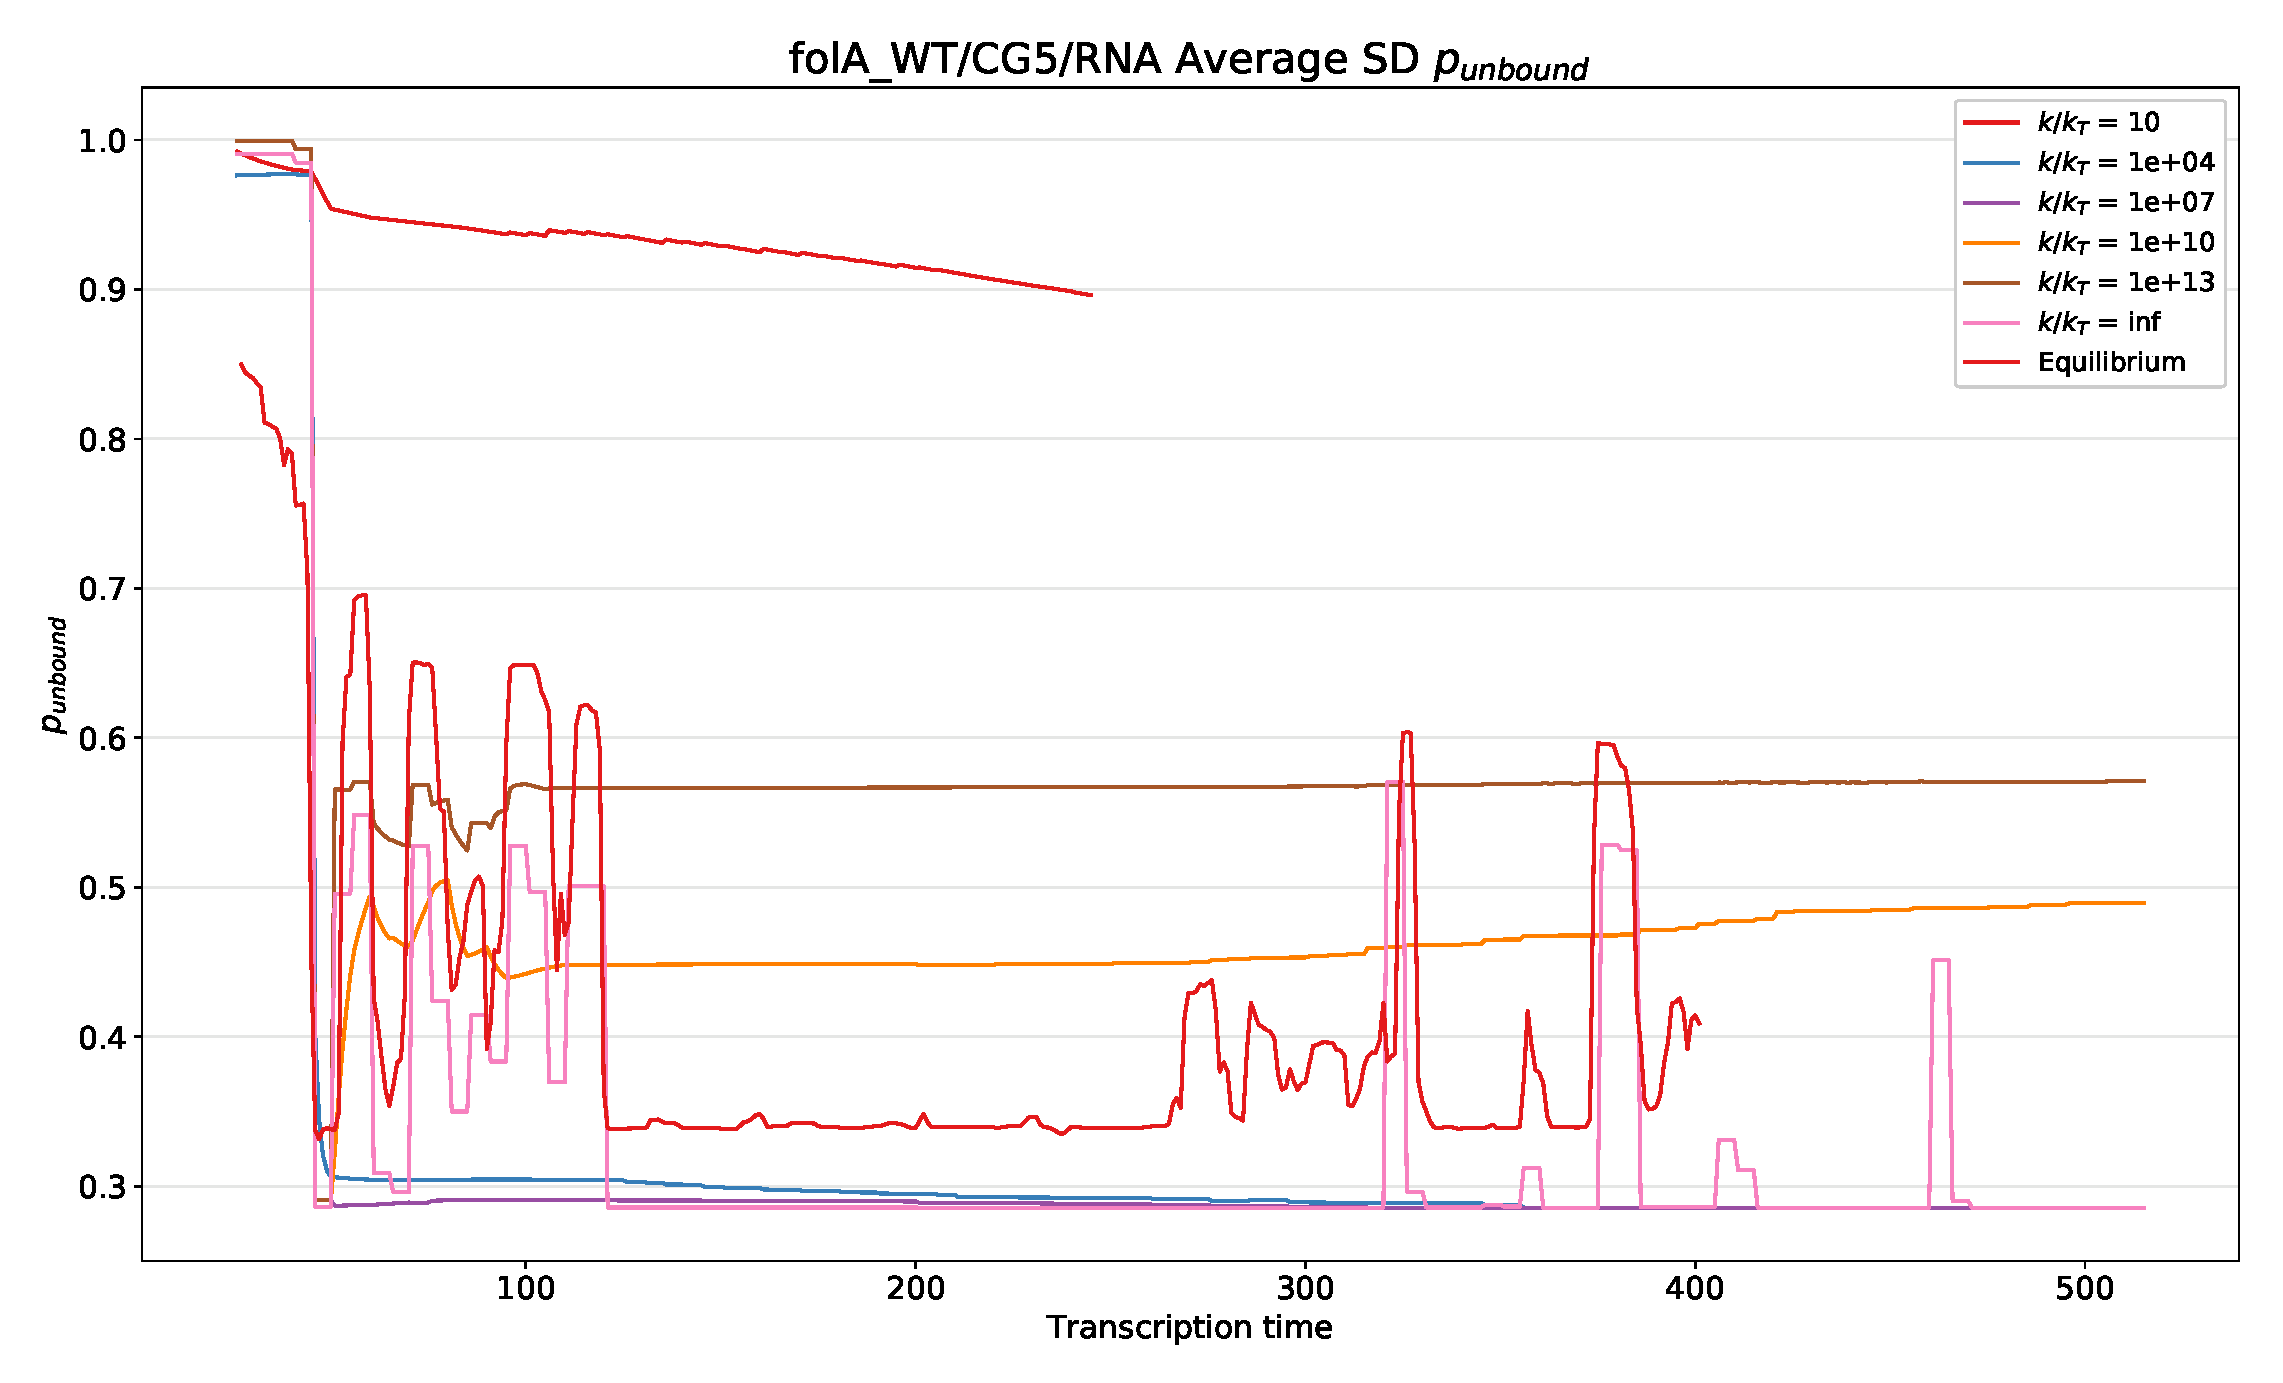
\includegraphics[width=\linewidth]{p_unbound/RNA_p_unbound_SD_k_tuning}
      \caption[]%
      {{\small folA\textsubscript{WT} average $p_{unbound}$ results.}}
    \end{subfigure}
   	\hfill
    \begin{subfigure}[t]{0.475\linewidth}
      \centering
      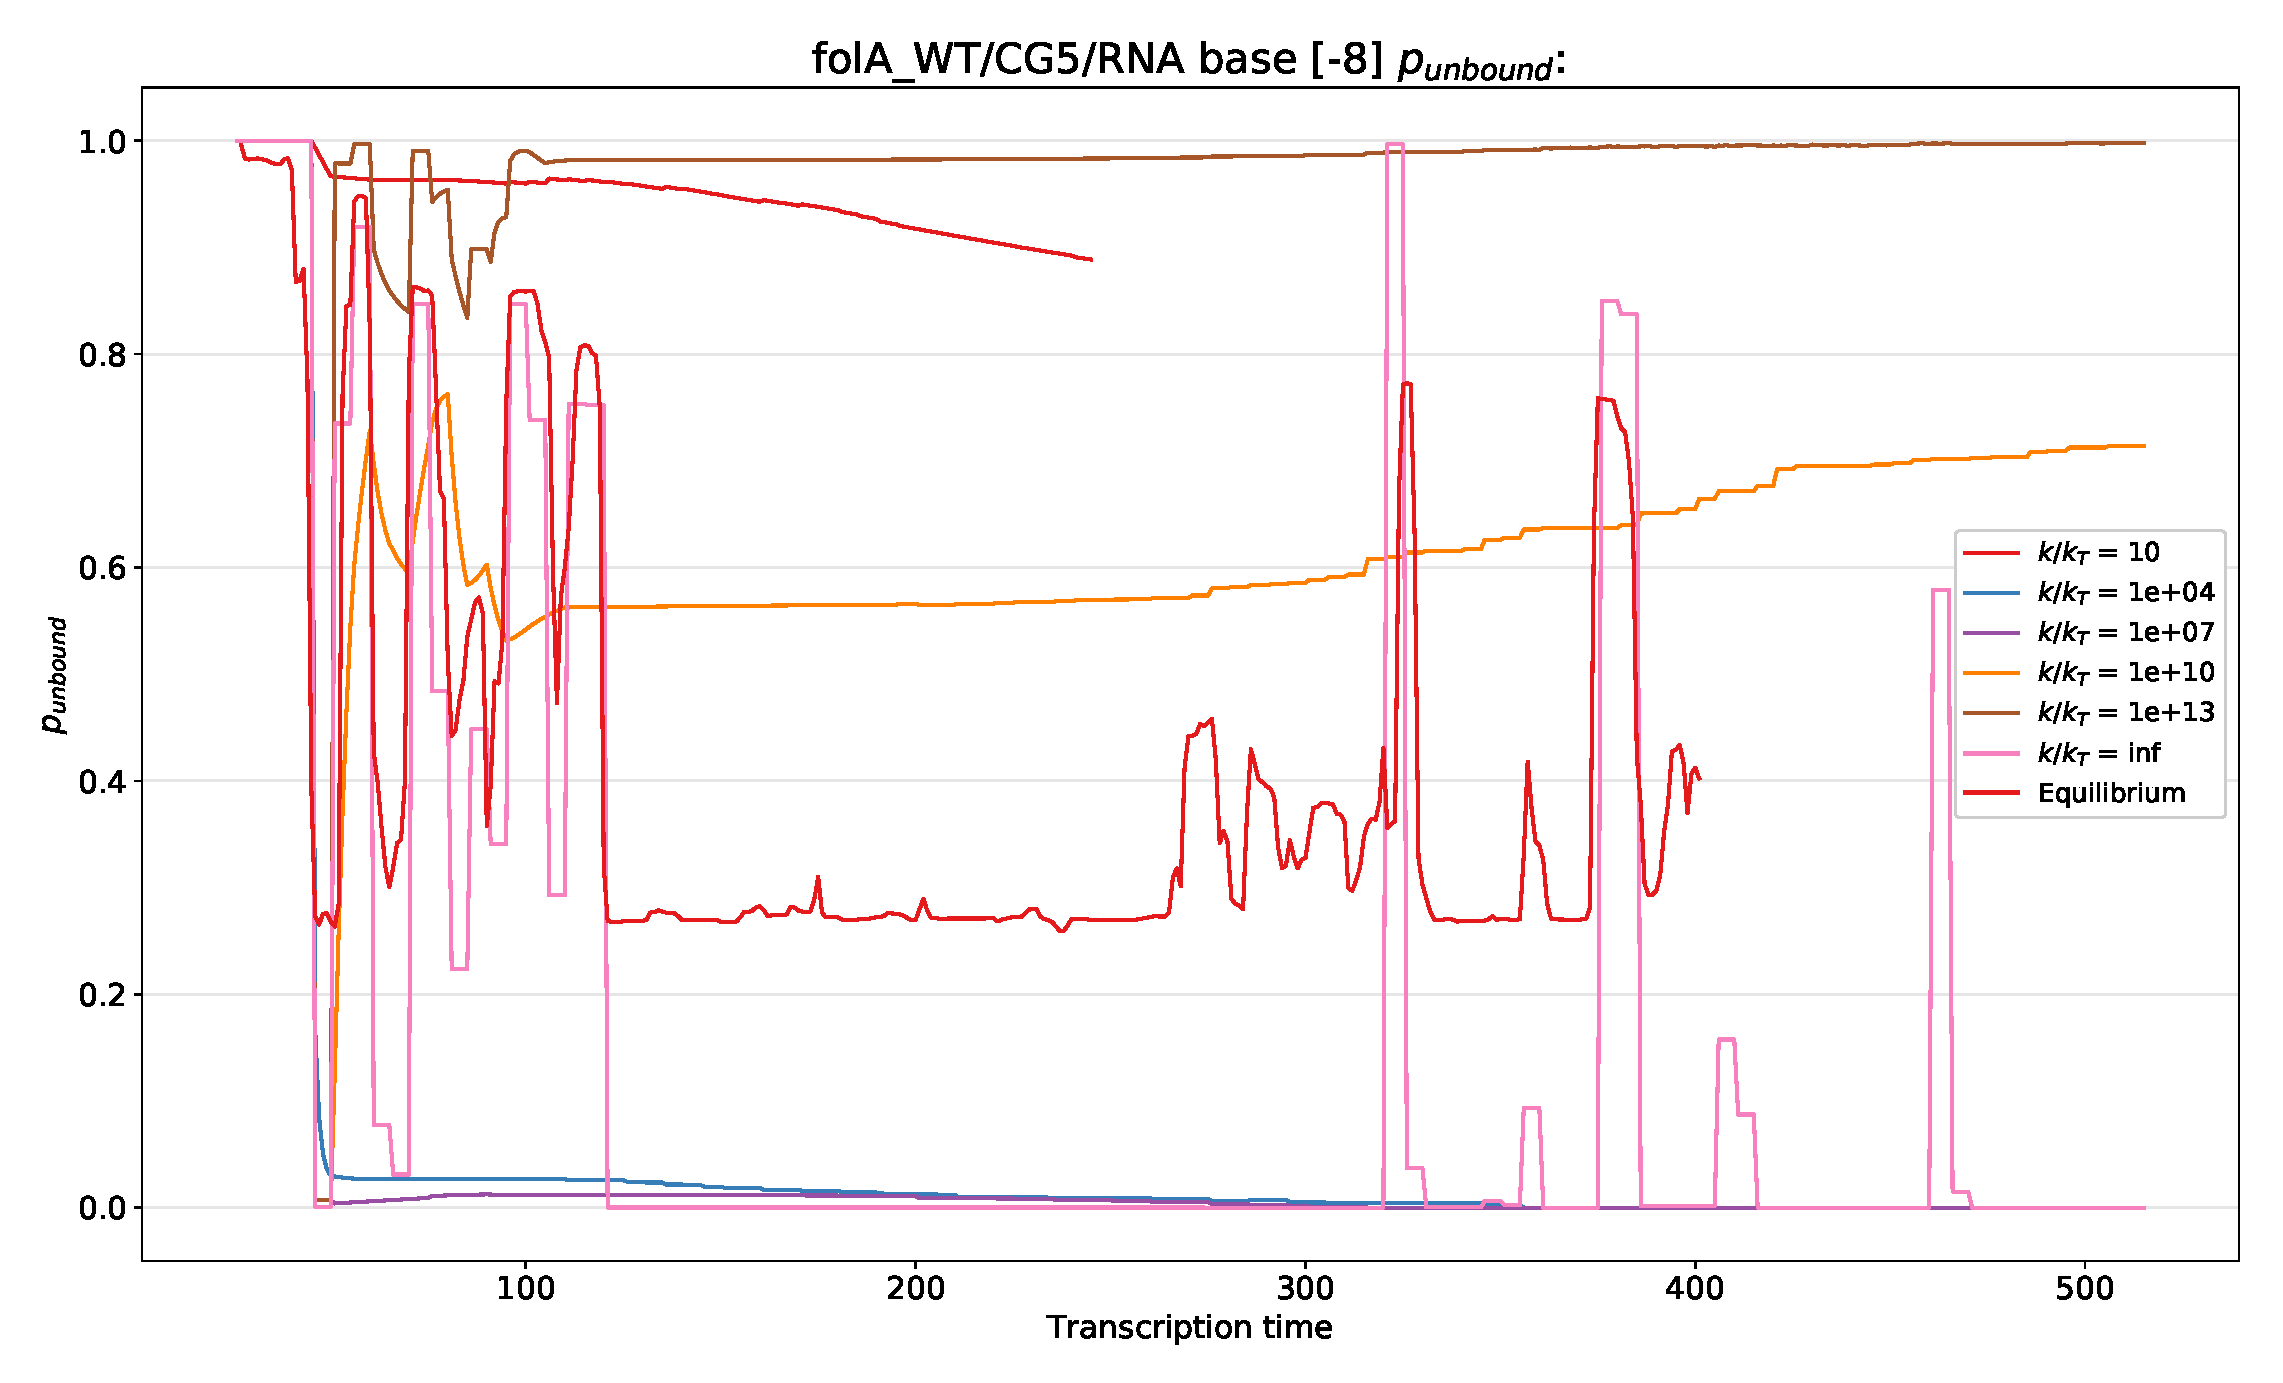
\includegraphics[width=\linewidth]{p_unbound/RNA_p_unbound_base[-8]_k_tuning}
      \caption[]%
      {{\small folA\textsubscript{WT} base[-8] $p_{unbound}$ results.}}
   	\end{subfigure}
   	\vskip\baselineskip
   	\begin{subfigure}[t]{0.475\linewidth}
      \centering
      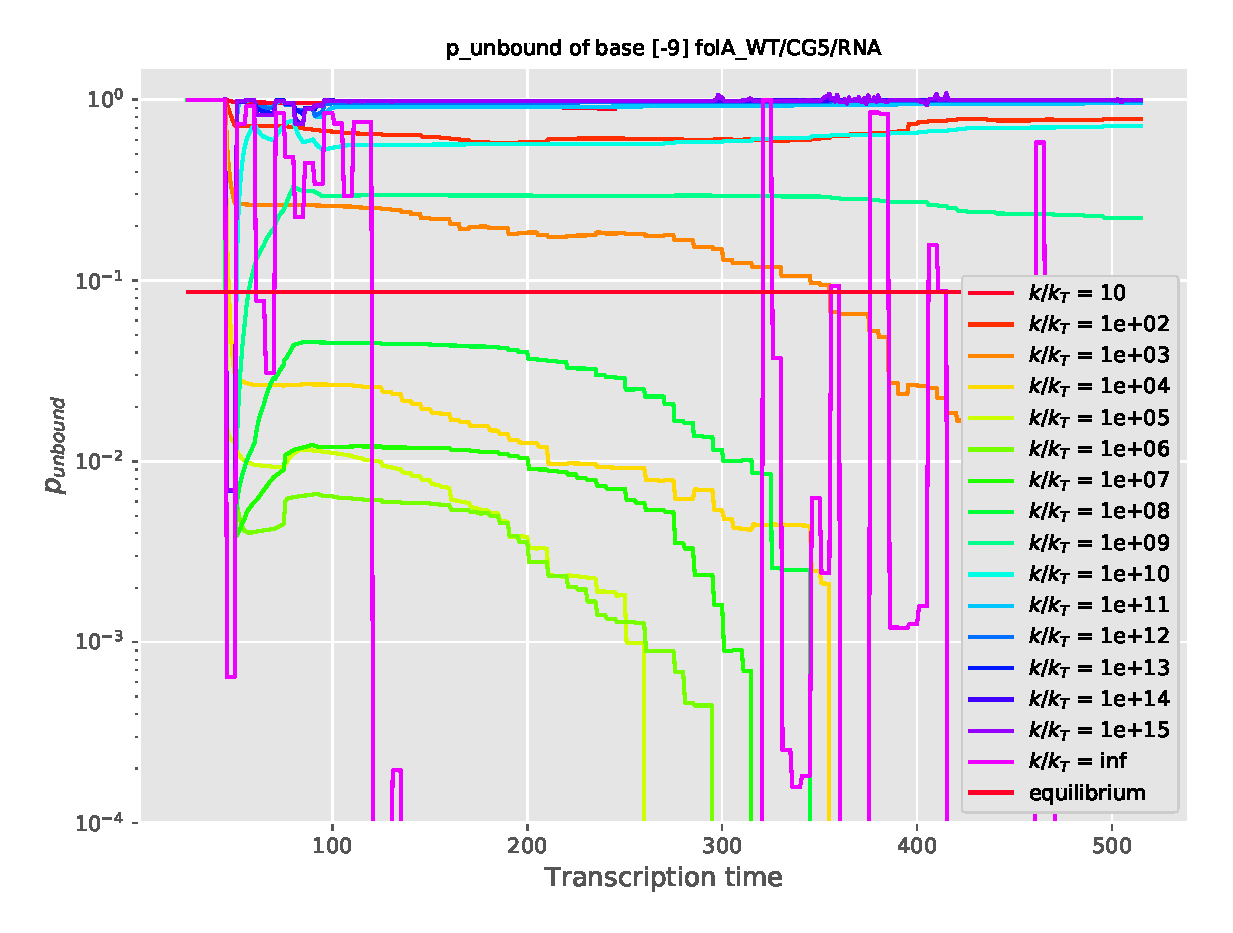
\includegraphics[width=\linewidth]{p_unbound/RNA_p_unbound_base[-9]_k_tuning}
      \caption[]%
   		{{\small Same as above, base -9.}}
    \end{subfigure}
   	\hfill
   	\begin{subfigure}[t]{0.475\linewidth}
      \centering
      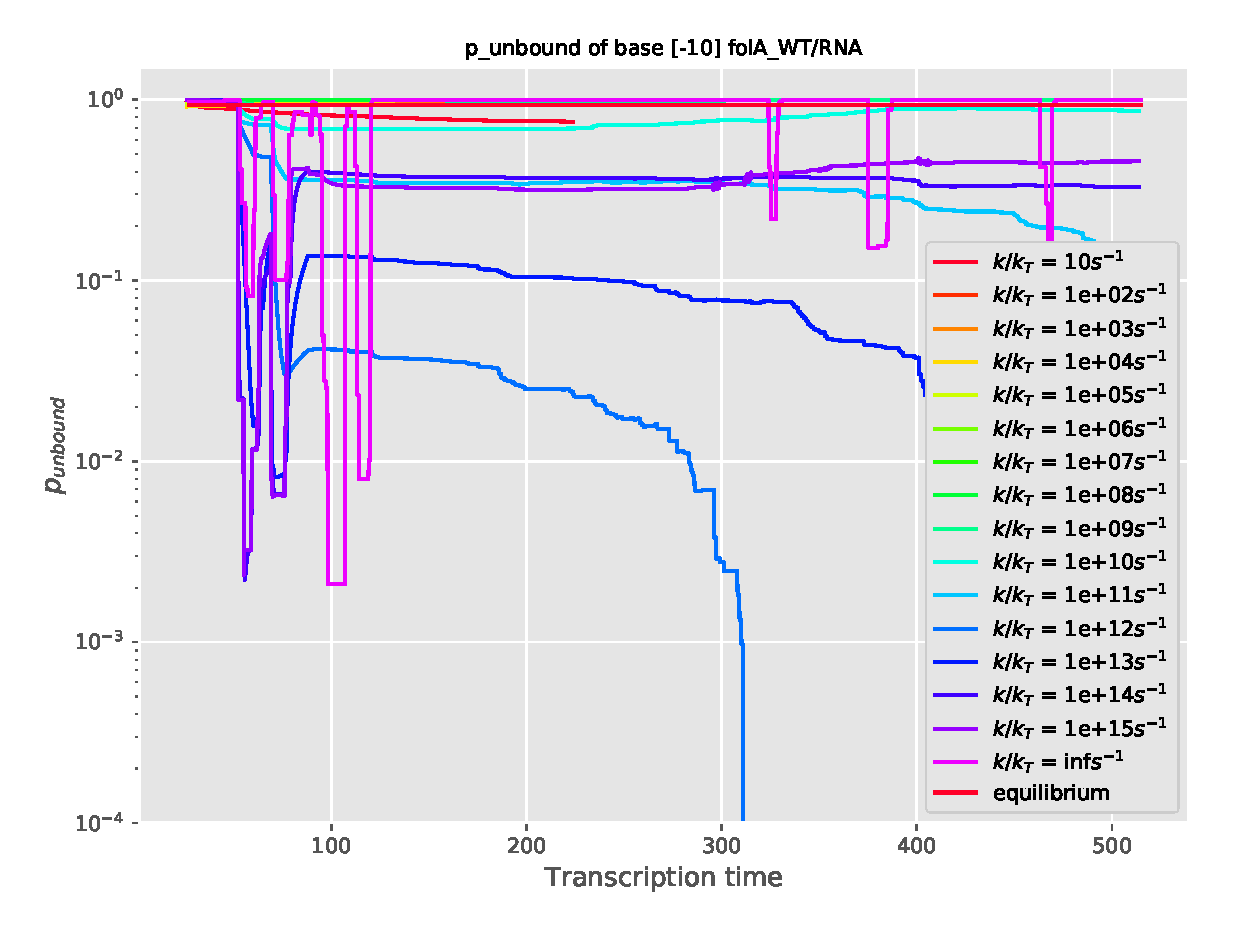
\includegraphics[width=\linewidth]{p_unbound/RNA_p_unbound_base[-10]_k_tuning}
      \caption[]%
      {{\small Same as above, base -10.}}
   	\end{subfigure}
    \vskip\baselineskip
   	\begin{subfigure}[t]{0.475\linewidth}
      \centering
      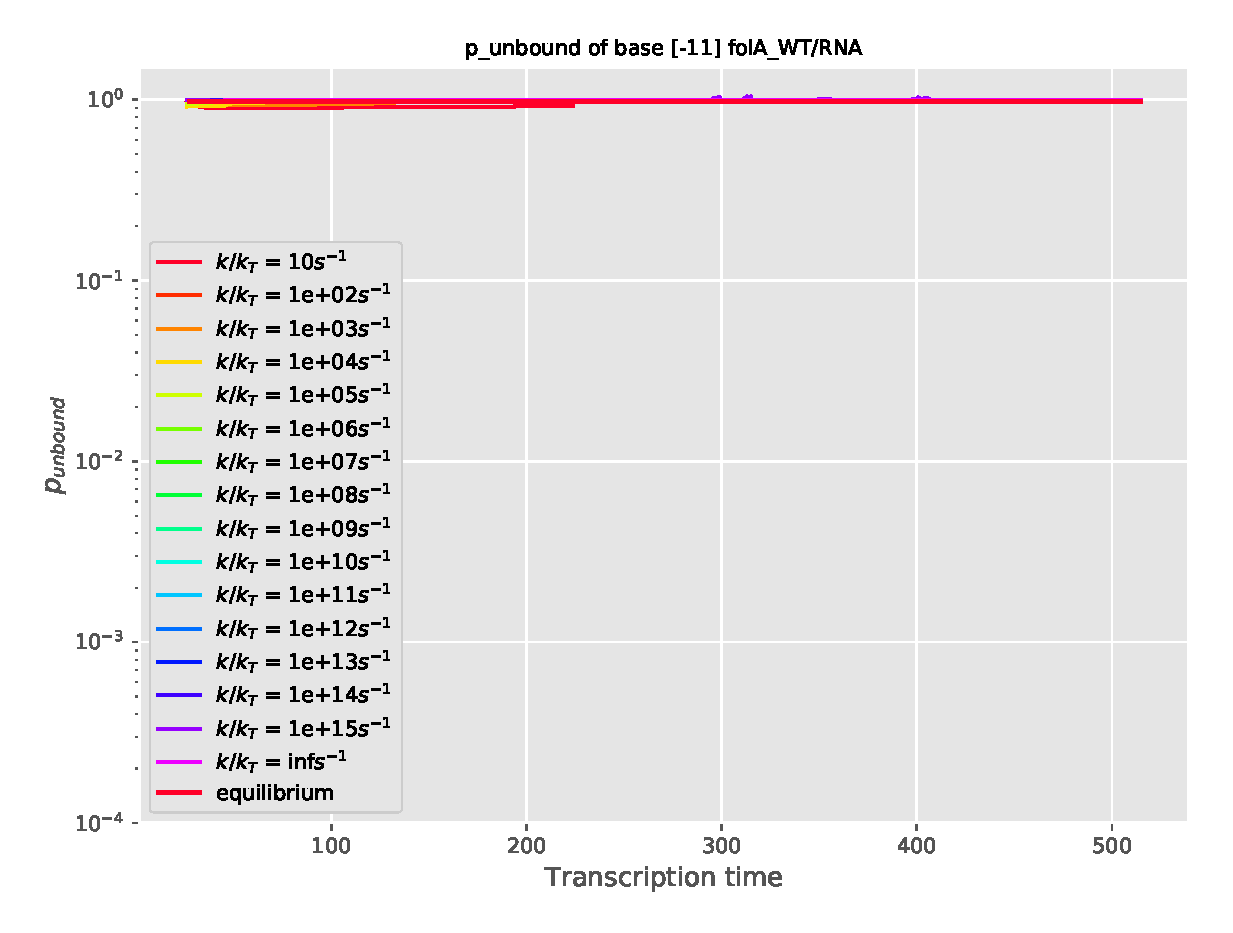
\includegraphics[width=\linewidth]{p_unbound/RNA_p_unbound_base[-11]_k_tuning}
      \caption[]%
   		{{\small Same as above, base -11.}}
    \end{subfigure}
   	\hfill
   	\begin{subfigure}[t]{0.475\linewidth}
      \centering
      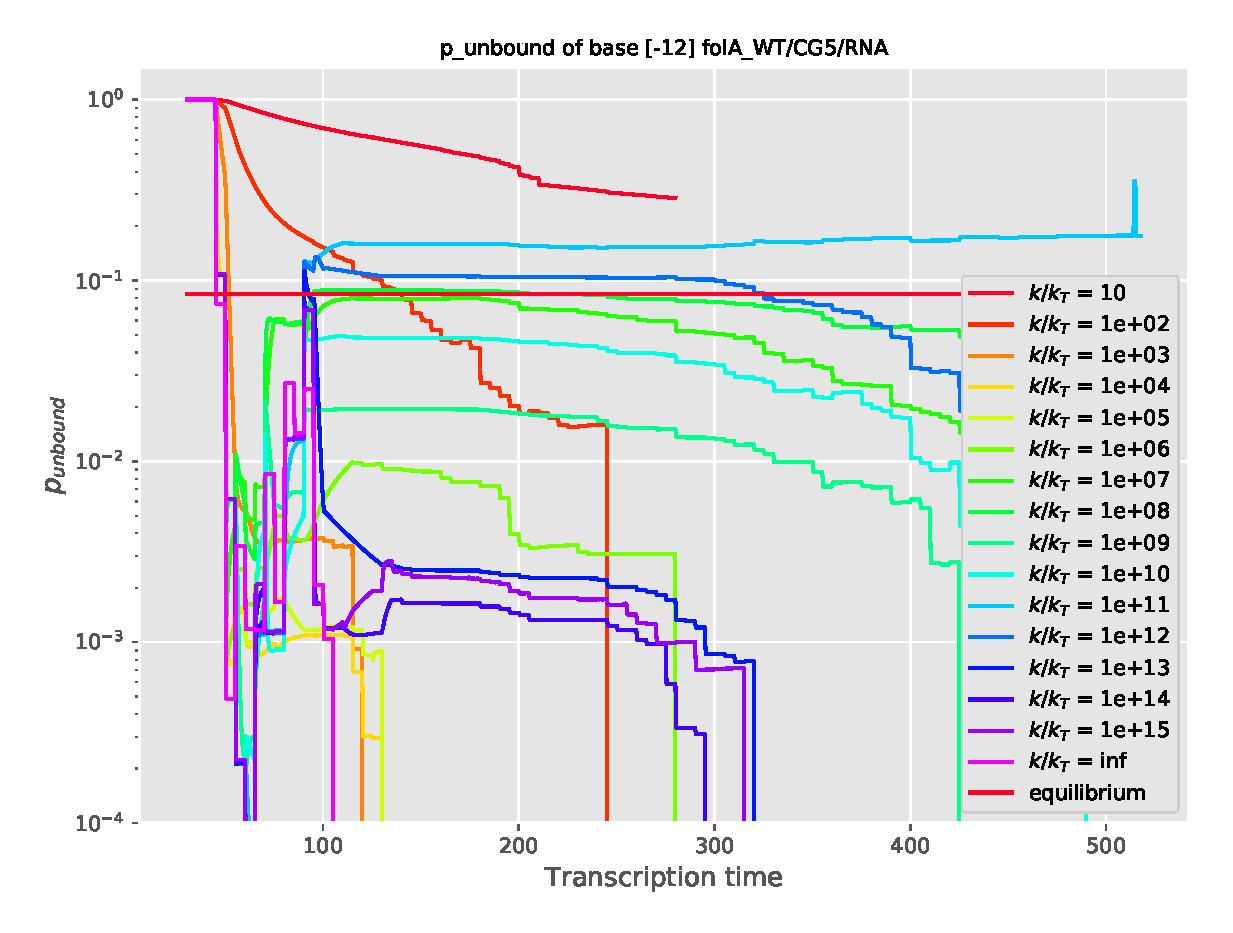
\includegraphics[width=\linewidth]{p_unbound/RNA_p_unbound_base[-12]_k_tuning}
      \caption[]%
      {{\small Same as above, base -12.}}
   	\end{subfigure}
    \vskip\baselineskip
   	\begin{subfigure}[t]{0.475\linewidth}
      \centering
      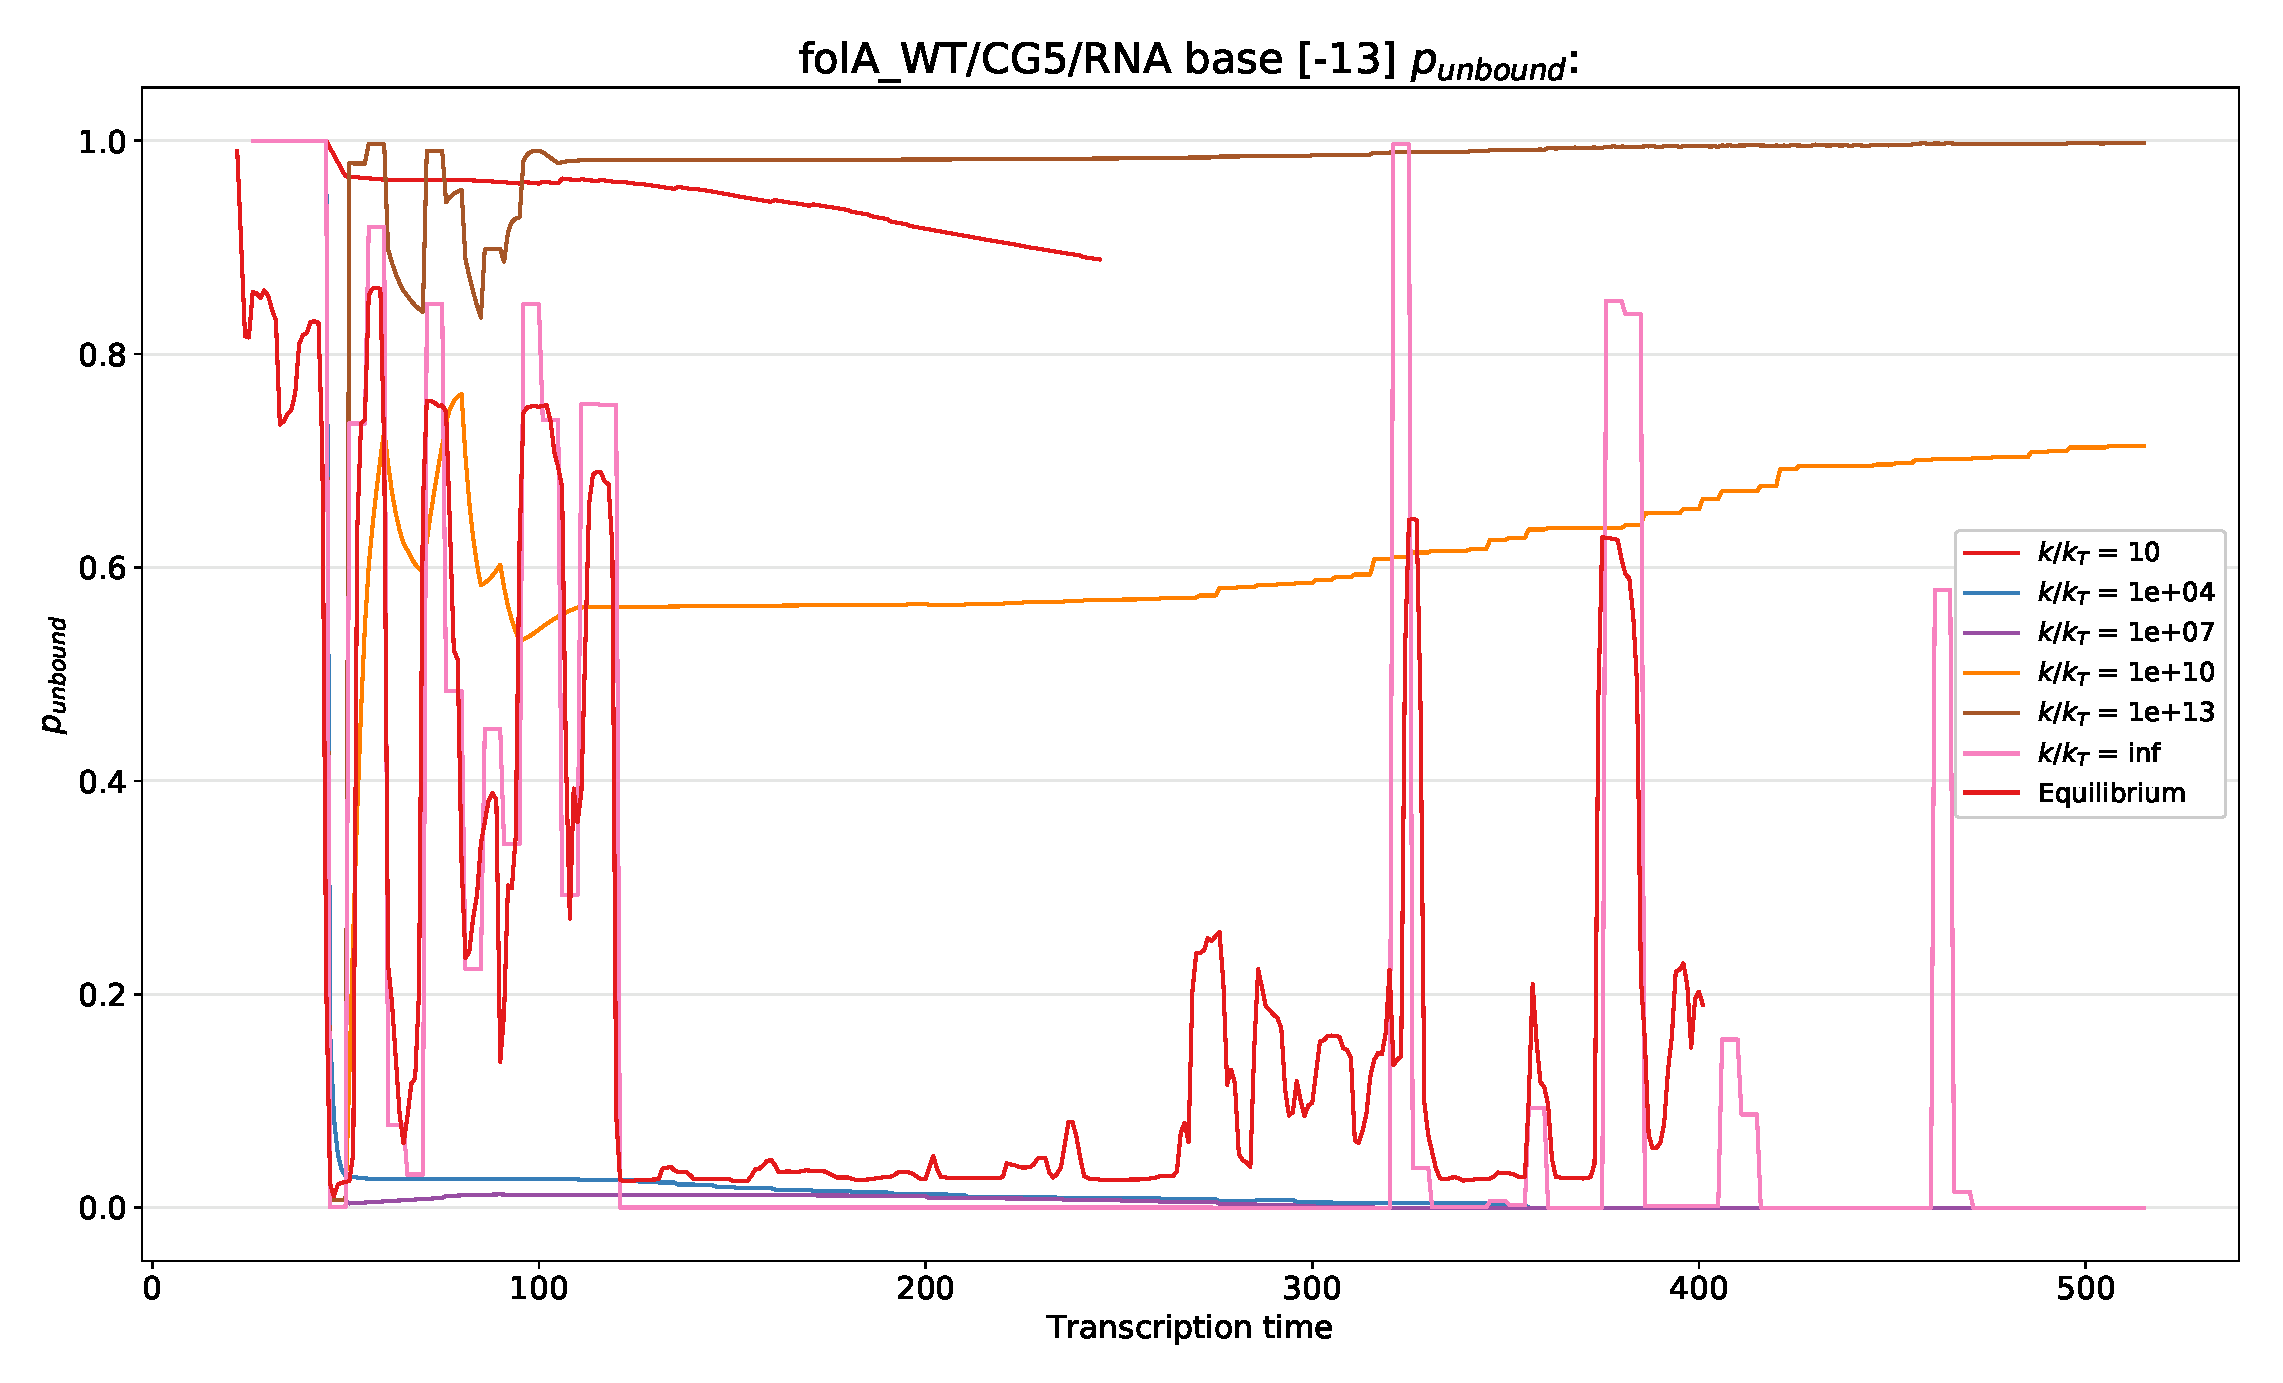
\includegraphics[width=\linewidth]{p_unbound/RNA_p_unbound_base[-13]_k_tuning}
      \caption[]%
   		{{\small Same as above, base -13.}}
    \end{subfigure}
   	\hfill
   	\begin{subfigure}[t]{0.475\linewidth}
      \centering
      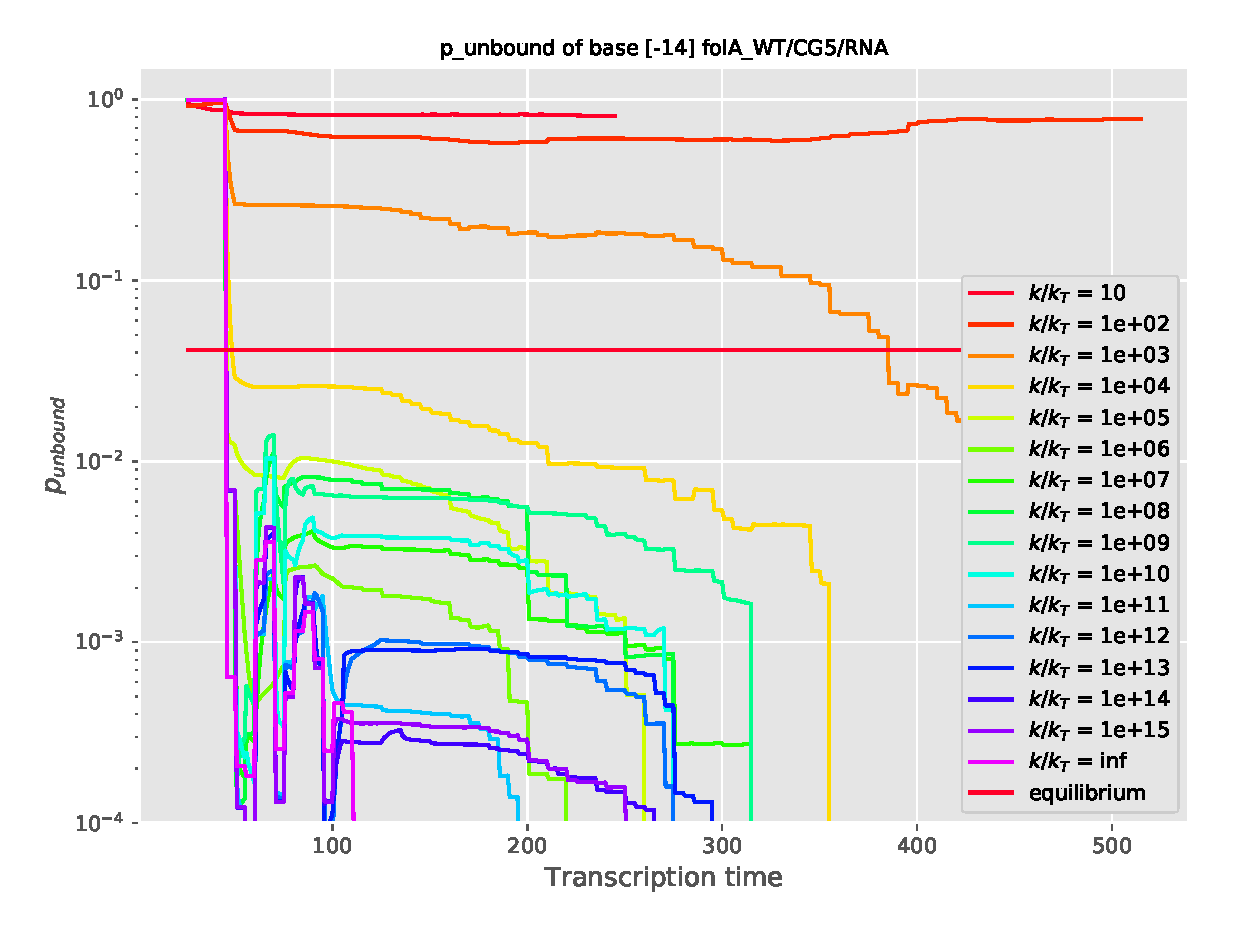
\includegraphics[width=\linewidth]{p_unbound/RNA_p_unbound_base[-14]_k_tuning}
      \caption[]%
      {{\small Same as above, base -14.}}
   	\end{subfigure}
    \caption[Average and single-base $p_{unbound}$ of SD sequence during co-transcription folding (after model optimization).]
    {\small Shine-Dalgarno average and single-base $p_{unbound}$ during co-transcription folding of folA\textsubscript{WT} mRNA (after model optimization).}
   	\label{fig:p_unbound_old}
\end{figure*}

\begin{figure}
\centering
\includegraphics[width=\linewidth]{folding_example_grey_compare.png}
\caption{Tentative kinetically important sub-optimum structures (dG = 0.7 kcal/mol).}
\label{fig:excp}
\end{figure}

\paragraph{Calibrate pre-exponential factor from TCSPC data.} We then resorted to the time scale of hairpin refolding to calibrate the absolute value of $k_0$. Specifically, we observed the relaxation corresponding to folding of the motif involving S-D sequence when $\frac{k_0}{k_T}$ is between $10^2$ and $10^3$ (Figure \ref{fig:populations});
 From TCSPC measurement data in \cite{}, we note that a similar 20 nt hairpin takes about 70 ns for refolding, commensurable to a scheme where $k_T=10^{9}\, s^{-1}$. Consequently, we estimated the value of pre-exponential factor to be $k_0=10^{11}$.

 \paragraph{Model optimization.} We observed that our model tends to overesitimate the flucuation of average $p_{unbound}$ when $k=\infty$, and some kinetic patterns were lost (for bases -11, -12 and -14). Specifically we found that for base -8 and base -9, our model gave identical results while for equilibrium nupack.ppairs calculation there was a overall upshift of $p_{unbound}$.

 Then we examined sub-optimal structures using nupack.subopt for sequence truncated at 150 nt, and found two tentative kinetically important structures between which free energy difference is 0.7 kcal (Figure \ref{fig:excp}). Coexistence of those sub-optimal structures instead of only the minimum free energy structure will possibly result in similar population dynamics as above but different $p_{unbound}$ at single base resolution. We also noticed that for mininum free energy motifs, base -11, -12 and -14 shared the same pairing patterns, meaning that $p_{unbound}$ on these bases has no response to motif population dynamics.

 We optimized foldon collection sets by incorporate sub-optimal structures with a energy gap of 1cal/mol by nupack.subopt algorithm and reconducted the computation for folA\textsubscript{WT}, setting ActivePool cutoff = 50 (Figure \ref{fig:p_unbound_new}). It's worth noting that after optimization predicted equilibrium $p_{unbound}$ values agreed much better with ensemble averaged $p_{unbound}$ (computed by nupack.ppairs, not shown here), and base-specificity of $p_{unbound}$ can be correctly reproduced.

\begin{figure*}[htp]
 \centering
 \includegraphics[width=\textwidth]{folA_local_population_evolution_summary_bin1}
 \caption[Population dynamics]{\small Population dynamics of folA\textsubscript{WT} S-D structrual motifs during co-transcriptional folding under varied $k_T$ (after calibration and model optimization).}
 \label{fig:populations_revised}
\end{figure*}

\begin{figure*}
    \centering
    \begin{subfigure}[t]{0.475\linewidth}
      \centering
      \includegraphics[width=\textwidth]{p_unbound_new/p_unbound_SD_k_tuning.png}
      \caption[]%
      {{\small Revised folA\textsubscript{WT} average $p_{unbound}$ results.}}
    \end{subfigure}
   	\hfill
    \begin{subfigure}[t]{0.475\linewidth}
      \centering
      \includegraphics[width=\textwidth]{p_unbound_new/p_unbound_base[-8]_k_tuning_linear.png}
      \caption[]%
      {{\small Revised folA\textsubscript{WT} base[-8] $p_{unbound}$ results.}}
   	\end{subfigure}
   	\vskip\baselineskip
   	\begin{subfigure}[t]{0.475\linewidth}
      \centering
      \includegraphics[width=\textwidth]{p_unbound_new/p_unbound_base[-9]_k_tuning_linear.png}
      \caption[]%
   		{{\small Same as above, base -9.}}
    \end{subfigure}
   	\hfill
   	\begin{subfigure}[t]{0.475\linewidth}
      \centering
      \includegraphics[width=\textwidth]{p_unbound_new/p_unbound_base[-10]_k_tuning_linear.png}
      \caption[]%
      {{\small Same as above, base -10.}}
   	\end{subfigure}
    \vskip\baselineskip
   	\begin{subfigure}[t]{0.475\linewidth}
      \centering
      \includegraphics[width=\textwidth]{p_unbound_new/p_unbound_base[-11]_k_tuning_linear.png}
      \caption[]%
   		{{\small Same as above, base -11.}}
    \end{subfigure}
   	\hfill
   	\begin{subfigure}[t]{0.475\linewidth}
      \centering
      \includegraphics[width=\textwidth]{p_unbound_new/p_unbound_base[-12]_k_tuning_linear.png}
      \caption[]%
      {{\small Same as above, base -12.}}
   	\end{subfigure}
    \caption[Average and single-base $p_{unbound}$ of SD sequence during co-transcription folding (after model optimization).]
    {\small Shine-Dalgarno average and single-base $p_{unbound}$ during co-transcription folding of folA\textsubscript{WT} mRNA (after model optimization).}
   	\label{fig:p_unbound_new}
\end{figure*}


\section{Results and discussion}
\subsection{Transcription rate dependence on co-transcriptional mRNA folding kinetics.}
We then tuned the RNA polymerase transcription rate away from physiological condition, from $k_T = 1 \, nt\times 10^{-7} \, s^{-1}$ to $k_T=1 \, nt \times 10^{7} \, s^{-1}$ and compared the behavior of $p_{unbound}$ during co-transcription folding (Figure \ref{fig:p_unbound_new}, a). It's worth noting that before the transcription of base 20, $p_{unbound}$ value of all kinetic schemes remained close to equilibrium asymptotic results, which was analogous to a scheme of infinitely slow transcription. Once downstream region is transcribed, however, the $p_{unbound}$ value started to diverge.

This divergence reflected an altered Shine-Dalgarno folding stability after the formation of downstream structures, allostericly shifting from a minima in local free energy surface to a sub-optimum which contributed to globally more stable secondary structures. The kinetic dependence was thus triggered by the barrier crossing dynamics between the local folding free energy minima to another favorable structure in the configuration space of longer mRNA intermediate segments.

\subsection{mRNA level - transcient $p_{unbound}$ correlation within a synonymous mutants library.}
We repeated GenoFold folding prediction for all synonymous sequences in \cite{}, which contains synonymous codon substitutions for gene folA and Adk in both N-terminal and downstream region. As a initial test we calculated the correlation between transcient averge Shine-Dalgarno $p_{unbound}$ when base 100 is transcribed and measured mRNA levels among the synonymous mutants library. Comparing to the equilibrium model (Figure \ref{fig:base100corr}, left) which predicted no $p_{unbound}$ dependence of mRNA level variation for sequences with synonymous substitution downstream in the coding region, the non-equilibrium model (Figure \ref{fig:base100corr}, right) can much better discern the sequence dependence of transcient S-D $p_{unbound}$ and desmonstrated a significant correlation between transcient S-D $p_unbound \,(base[100])$ and the log ratio of mRNA levels.

\begin{figure}[htp]
  \centering
  \includegraphics[width=\textwidth]{base100_corr.PNG}
  \caption{Correlation between transient average Shine-Dalgarno $p_{unbound}$ when base 100 is transcribed and measured mRNA levels.}
  \label{fig:base100corr}
\end{figure}

Then we intended to capture the characteristic time scale of ribosome binding during transcription. We varied the snapshot transcription time taken to calculate transient $p_{unbound}$ and trancription rate $k_T$, then summarized the result of measured mRNA level - transient S-D $p_{unbound}$ correlation coefficient (pearson R) at given snapshot transcription times and $k_T$ (Figure \ref{fig:timeCorrMatrix}). Strikingly we noticed that significant correlation could be observed only within diagonal elements, indicating kinetic schemes with commensurable snapshot and transcription time scale, reflecting a coupling between ribosome binding. This is consistent with the fact that mRNA levels are largely insensitive to codon substitutions when folA synonymous codon variants are cloned under the T7 rather than pBAD/E. Coli RNAP system. In addition to the discussion in \cite{}, it offered an complementary hypothesis that variation of ribosome binding affinities among synonymous codon mutants quantitatively diffrent between fast and slow transcription scheme, resulting in altered measured protein levels.

\begin{figure}[htp]
  \centering
  \includegraphics[width=360pt]{timeCorrMatrix.PNG}
  \caption{Correlation coefficients between S-D averaged transcient $p_{unbound}$ and mRNA level variation correlation in various transcription-ribosome binding kinetic schemes.}
  \label{fig:timeCorrMatrix}
\end{figure}

More detailedly we analyzed mRNA level - transient S-D averaged $p_{unbound}$ correlation after each base is transcribed with a bin of 5 bases (Figure \ref{fig:allCorrMatrix}). Significant correlation could be observed in N-terminal region over all kinetic schemes, which is possibly because of the similar refolding kinetics of N-terminal region. In contrast, only physiological kinetic scheme ($k_T=10 nt/s$) showed a strong correlation after the transcript is elongated to downstream region. On the contrary, equilibrium model showed no significant correlation downstream, reiterating that transcient S-D sequence accessibility variation is not an artifact of equilibrium folding stability.

\begin{figure}[htp]
  \includegraphics[width=550pt]{mRNA-p_unbound(transcript_length)correlation_test_n+nc+cterm_SD_5-200_091118.png}
  \caption{Correlation between transient S-D averaged $p_{unbound}$ - mRNA level when given bases is transcribed under different log ratio of $k_T$. Correlation is most significant when down-stream region is released under physiological transcription rate.}
  \label{fig:allCorrMatrix}
\end{figure}
%\cite{Jacobs2018,Chaudhury2010,Vanden-Eijnden2010,Metzner,Krivov}
\section{Future Plan}
\paragraph{1} Obtain more accurate S-D accessibility indicator by calculating local domain unfolding free energy from transcient secondary structure distribution.
\paragraph{2} Develop kinetic models to address the mechanism underlying translation initiation rate – mRNA level correlation, including Rho-dependent transcription termination and RNA degradation.
\paragraph{3} Use genome and species-wide analysis to investigate the effect of transcription - translation initiation coupling on evolutionary selection pressure on codon usage.

\small
\bibliographystyle{unsrt}
\bibliography{ref}

\end{document}
